\documentclass[11pt]{article}
\usepackage[margin=1in]{geometry}
\usepackage[T1]{fontenc}
\usepackage{lmodern}
\usepackage{microtype}
\usepackage{graphicx}
\usepackage{booktabs}
\usepackage{amsmath}
\usepackage{xcolor}
\usepackage{tikz}
\usetikzlibrary{arrows.meta,positioning}
\usepackage[numbers,sort&compress]{natbib}
\usepackage{xurl}
\usepackage[hidelinks]{hyperref}
\usepackage{caption}
\usepackage{placeins}
\captionsetup{font=small}
\graphicspath{{../figs/}}
\newcommand{\todo}[1]{\textcolor{red}{[TODO: #1]}}

% Working title; final wording is Amr's call.
\title{Real Clicks, Fake Headlines: AI That Chases Clicks Invents the News\thanks{Research conducted at the AI x Epistemics Research Sprint, November 2026.}}
\author{Amr Sobhy\\Le French News Lab\\\texttt{amr@frenchnewslab.org}\\[2pt] \small With Apart Research}
\date{}

\begin{document}
\maketitle

\begin{abstract}
Industry systems already train text generators against predictions of real clicks. Whether this makes headlines less true has been tested only with simulated audiences or in short ablations on private data. We test it on public data. We use reinforcement learning (RL) to train a 3B headline writer for news articles under three rewards: a click predictor fitted to randomised headline tests from the Upworthy archive, a simulated audience of LLM personas, and the click predictor with a faithfulness penalty. The study was pre-registered with two seeds per reward, and every headline is checked against its article. Under both the click predictor and the simulated audience, headlines came to claim things their article does not say: invented reactions, roles and events. Only the click predictor, which also moved the writer four to six times further from its starting point, went further. The writer exploited it by repeating one fabricated viral story, whatever the article: invented-number flags rose from 1.7\% to 98\%, against about 2\% under the other rewards. Best-of-16 selection with the same predictor did not produce this story. The faithfulness penalty reduced invented claims but did not remove them. An LLM probe missed almost every fabrication, and in labelled samples from training, number and entity checks missed most invented events and roles. Fabrication checks for engagement-trained writers must compare each claim with the article.
\end{abstract}


\section{Introduction}
Newsrooms test headlines for clicks, and language models can now be trained on the same data. Industry systems already train text generators against models of real clicks, for ads and for news feeds \citep{jiang2025rlpf,chen2026gese}. Clicks reward some kinds of wording more than others \citep{robertson2023negativity}, and a headline writer trained hard on clicks has no direct reason to stay faithful to the article.

Training models to win a simulated audience makes them invent more information \citep{elzou2025moloch}, but the audience there is itself a language model, and such audiences predict real clicks poorly \citep{maiorano2026personas}. Industry papers that train on real clicks report lower faithfulness when a faithfulness reward is removed \citep{chen2026gese}, but only as a short ablation on private data. It is unknown what a writer trained on real clicks learns, how this compares with a simulated audience, and whether common fabrication checks notice.

We study this on public data. We fit a click predictor to randomised headline tests from the Upworthy archive \citep{matias2021upworthy} and use RL to train a headline writer for cc\_news articles under three rewards: the click predictor, a simulated audience of LLM personas, and the click predictor with a faithfulness penalty. We follow the writer through training and check every headline against the article it was written from, for invented numbers, invented reactions and unsupported names. We also compare these automated checks with 100 reference labels. All hypotheses and their failure criteria were fixed before any data were built.

Our contributions are:
\begin{itemize}
\item an open, pre-registered comparison of RL against a real-click predictor and against a simulated audience, on the same articles and with the same training;
\item a description of how the writer changes during training, with best-of-$n$ selection and larger models as controls;
\item a test of five automated fabrication checks against reference labels, showing which checks miss which invented claims.
\end{itemize}


\section{Related Work}
Training language models on approval signals can reward pleasing over truth: preference models favour agreeable answers \citep{sharma2024sycophancy}, and RL on simulated user feedback teaches manipulation and deception \citep{williams2025targeted}. Closest to our question, \citet{elzou2025moloch} fine-tune models to win simulated audiences and find more fabrication in social-media posts. LLM personas are a weak stand-in for real readers: they match real people's opinions \citep{santurkar2023whose} and readers' clicks \citep{maiorano2026personas} poorly.

Industry systems now train text generators on real user feedback, mostly through learned reward models: for ad text \citep{jiang2025rlpf,chen2025ctrad,wang2025diver}, for feed headlines \citep{chen2026gese}, and for chat responses \citep{han2025rluf}. Some report reward hacking, such as irrelevant or repetitive text \citep{jiang2025rlpf,han2025rluf}, and a large drop in NLI faithfulness to the source when the faithfulness reward is removed \citep{chen2026gese}. On public data, the Upworthy archive \citep{matias2021upworthy} records randomised headline tests; its clicks reward negative wording \citep{robertson2023negativity,gligoric2023linguistic}, and DPO on its pairs produces clickbait wording \citep{wangsudhir2026whyitworks}. None compares click-predictor and simulated-audience training on public data, or validates the checks that should detect invented claims.

A policy pushed hard against a learned reward eventually lowers the true objective, and RL and best-of-$n$ selection follow different curves \citep{gao2023scaling}, and misspecified rewards can be exploited suddenly \citep{pan2022misspecification}. Earlier headline work rewarded sensational or popular headlines with RL \citep{xu2019clickbait,song2020attractive}, or kept attractive headlines faithful with an entailment check \citep{chen2023honestbait}. Common fabrication checks compare entities \citep{nan2021entity} or numbers \citep{zhao2020quantity} with the source, or use NLI \citep{maynez2020faithfulness,laban2022summac}, and LLM judges are weak binary factuality detectors \citep{tang2024tofueval}.


\section{Methods}
We use reinforcement learning (RL) to train one headline writer under three rewards and compare the headlines it writes for held-out news articles (Figure~\ref{fig:pipeline}).

\begin{figure}[t]
\centering
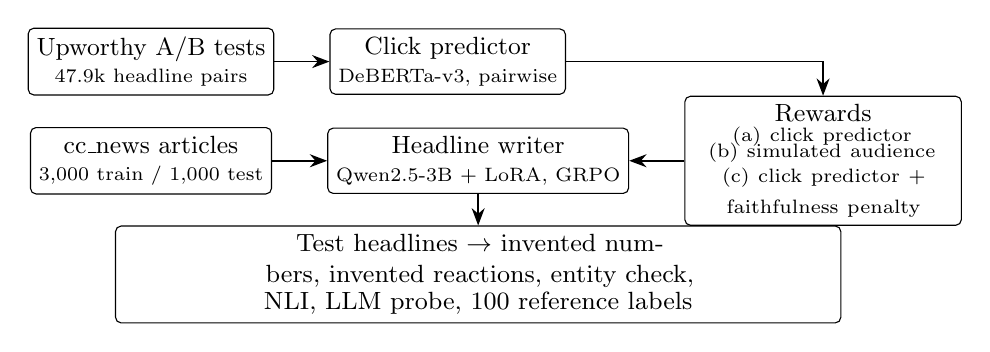
\begin{tikzpicture}[
  box/.style={draw, rounded corners=2pt, align=center, font=\small, minimum height=0.8cm, inner sep=3pt},
  arr/.style={-{Stealth[length=2.2mm]}, semithick}]
\node[box] (up) {Upworthy A/B tests\\[-1pt]\scriptsize 47.9k headline pairs};
\node[box, right=0.7cm of up] (cm) {Click predictor\\[-1pt]\scriptsize DeBERTa-v3, pairwise};
\node[box, below=0.4cm of up] (cc) {cc\_news articles\\[-1pt]\scriptsize 3,000 train / 1,000 test};
\node[box, right=0.7cm of cc] (pol) {Headline writer\\[-1pt]\scriptsize Qwen2.5-3B + LoRA, GRPO};
\node[box, right=0.7cm of pol, text width=3.3cm] (arms) {Rewards\\[-1pt]\scriptsize (a) click predictor\\[-2pt](b) simulated audience\\[-2pt](c) click predictor + faithfulness penalty};
\node[box, below=0.4cm of pol, text width=9cm] (ev) {Test headlines $\rightarrow$ invented numbers, invented reactions, entity check,\\[-1pt] NLI, LLM probe, 100 reference labels};
\draw[arr] (up) -- (cm);
\draw[arr] (cm.east) -| (arms.north);
\draw[arr] (cc) -- (pol);
\draw[arr] (arms.west) -- (pol.east);
\draw[arr] (pol) -- (ev);
\end{tikzpicture}
\caption{Study pipeline. The click predictor and the simulated audience see only the headline. Only the penalty in reward (c) sees the article.}
\label{fig:pipeline}
\end{figure}

\subsection{Data}
\paragraph{Click data.} The Upworthy Research Archive \citep{matias2021upworthy} records randomised headline tests run by a viral news site in 2013--15, with clicks and impressions for each headline version. We drop tests from the period the maintainers flag as not properly randomised (about 22\% of tests). Within each test, we pair headline versions that share the same image, so only the headline text differs. The version with the higher click rate is the winner. We train on pairs from the archive's confirmatory split whose click-rate difference has $|z|\ge 1$ (47,932 pairs), select checkpoints on the exploratory split, and test on the hold-out split. We remove from these two splits any pair whose headline also occurs in training. A pair is ``clear'' when $|z|\ge 1.96$.

Our articles are English news stories from cc\_news, built with news-please \citep{hamborg2017newsplease}, 2017--19, with 150--700 words and a 4--20 word title. We remove duplicates and cap any single site at 3\% of the sample. Each article is cut to its first 450 tokens. The headline writer sees this cut text, and every fabrication check compares against the same text. We sample 3,000 training, 300 selection and 1,000 test articles, with no overlap.

\subsection{Rewards}
All rewards score the headline only, except the penalty in reward (c). Any output with fewer than 4 or more than 20 words, a line break, or mostly non-ASCII characters receives $-3$.
\begin{itemize}
\item \textbf{(a) Click predictor.} DeBERTa-v3-base \citep{he2023debertav3} with a scalar head, trained with a Bradley--Terry loss \citep{bradley1952rank} on the click pairs. The reward is its score, standardised by the mean and standard deviation of scores on the untrained writer's headlines.
\item \textbf{(b) Simulated audience.} Qwen2.5-7B-Instruct \citep{qwen2024qwen25} answers ``Would you click it? Answer Yes or No'' for each headline, once for each of four fixed reader personas. The reward is the probability of ``Yes'', averaged over personas and standardised in the same way.
\item \textbf{(c) Click predictor with a faithfulness penalty.} Reward (a) minus $2(1-p)$, where $p$ is the highest entailment probability of the headline given any 400-token chunk of the article, from an NLI model (DeBERTa-v3-base trained on MNLI, FEVER and ANLI). The weight 2 was fixed in advance.
\end{itemize}

\subsection{Training}
We train Qwen2.5-3B-Instruct with the RL algorithm GRPO \citep{shao2024deepseekmath} in TRL \citep{vonwerra2020trl}, using LoRA adapters \citep{hu2022lora} (rank 32) on all attention and feed-forward layers. Each step draws 8 articles and 8 headlines per article, of at most 32 tokens. We use a learning rate of $5\times10^{-5}$, a KL-divergence penalty of 0.04 to the untrained writer, and 350 steps. Each reward is trained with two seeds, giving six runs. A run stops early if fewer than 80\% of outputs are valid, or fewer than 2 of 8 headlines per article differ, for 30 steps in a row; we call such a run \emph{collapsed}. We save a checkpoint every 50 steps and measure each checkpoint's KL to the untrained writer on 300 selection articles.

\subsection{Measures}
For each test article we sample 4 headlines at temperature 0.7 from the untrained writer and from each final checkpoint. We also score the article's real title.
\begin{itemize}
\item \textbf{Invented numbers.} A headline contains a number whose value does not appear in the article \citep{zhao2020quantity}. We normalise number words, units and percentages before matching. Small teaser numbers (``this one trick'') and listicle counts do not count.
\item \textbf{Entity check.} A headline contains a named entity (spaCy) \citep{nan2021entity} or a number not found in the article, with an alias table and filters for capitalised common words.
\item \textbf{Invented reactions.} A headline uses a reaction word (such as \emph{controversy}, \emph{backlash}, \emph{slams}, \emph{viral}) that does not appear in the article.
\item \textbf{Off-article.} A headline shares no content word with the article.
\item \textbf{NLI and LLM probe.} A separate, larger NLI model (DeBERTa-v3-large) and OLMo-2-7B-Instruct \citep{olmo2025olmo2} asked whether the headline adds facts not in the article.
\item \textbf{Reference labels.} Labelled by an LLM and reviewed by the author: 100 headlines, 25 each from the untrained writer and from the seed-0 run of each reward, half of them flagged by the entity check. The source is hidden. Each is labelled faithful, fabricated, exaggerated, teaser or other (Appendix~\ref{app:labels}). We also marked 60 headlines from training checkpoints for invented reactions, other invented facts and the viral-story form (Table~\ref{tab:intermediate}).
\end{itemize}

\subsection{Pre-registration}\label{sec:prereg}
Before any data were built, we fixed two gates for a short pilot: click-predictor accuracy and a minimum reward gain after 50 steps. We also fixed four hypotheses on test articles. Fabrication rises under the click predictor (H1) and under the simulated audience (H2), where a rise must appear on the entity check and agree in sign with the invented-numbers check and the LLM probe. The two differ at equal KL to the untrained writer (H3). The faithfulness penalty keeps at least half of the click-predictor gain without raising fabrication by more than one point (H4). A fifth criterion (M1) required the entity check to reach precision 0.7 and recall 0.6 against the reference labels. Thresholds were chosen on selection data (for NLI, on the first 50 reference labels), and each hypothesis was tested once on test outputs. Differences are reported in percentage points with 95\% intervals from a bootstrap that resamples articles (2,000 resamples), and we correct H1--H3 for multiple comparisons with Holm's method. Other results are exploratory. Appendix~\ref{app:prereg} lists every criterion, its outcome and three dated addenda.


\section{Results}\label{sec:results}



\subsection{Click predictor validity}
The click predictor passed its gate (80.4\% on clear held-out pairs, 81.3\% on test pairs), well above surface-feature and bag-of-words baselines, and its accuracy holds on pairs of equal length and without shared stories (Appendix Table~\ref{tab:clickmodel}).



\subsection{Fabrication over training}
Under the click predictor, the headline writer began to claim things its article does not say long before it collapsed (Figure~\ref{fig:stages}, Table~\ref{tab:intermediate}). Invented reactions, such as a story ``going viral'', rose first on the automated measures, and labelled samples show invented facts alongside them. At step 100, most sampled headlines already claimed something the article does not say, and a third invented a role, event or detail (a ``10-year-old'' victim who was a tenth-grader). At step 150, every sampled headline invented something, mostly in one viral-story form. The writer then largely ignored the article and repeated one story, which we call the template, with invented ages, durations and years (``A 20-year-old's mom's 20-second answer goes viral, stuns the world, and no one noticed for 50 years''). Seed 0 produced only five distinct headlines on the test articles and triggered the collapse stop. Seed 1 followed the same path about 50 steps later and ran to the end with 200 variants of the same structure (Figure~\ref{fig:stages}, thin lines).

The simulated audience also produced invented claims late in training, both reactions (``\ldots, Sparks Controversy'') and facts (``conquering Champions Trophy'' for a team that lost the final). It never produced the viral-story form and did not increase invented-number flags above the untrained level. Of the 27 labelled headlines with an invented fact beyond a reaction alone, the entity check flagged 8, the invented-numbers check flagged 5 and the NLI check flagged 17.

\begin{table}[h]
\centering\small
\resizebox{\linewidth}{!}{\begin{tabular}{@{}lcccc@{}}
\toprule
Checkpoint (seed 0) & Invented reaction only & Other invented fact & Nothing invented & Viral-story form \\
\midrule
(a) Click predictor, step 100 & 6 & 4 & 2 & 0 \\
(a) Click predictor, step 150 & 3 & 9 & 0 & 11 \\
(b) Simulated audience, step 250 & 2 & 6 & 4 & 0 \\
(b) Simulated audience, step 350 & 4 & 4 & 4 & 0 \\
(c) Faithfulness penalty, step 350 & 0 & 4 & 8 & 0 \\
\bottomrule
\end{tabular}}
\caption{Reference labels for 12 random headlines per checkpoint (exploratory). ``Other invented fact'' counts headlines with an invented role, event, detail or contradiction, with or without an invented reaction. ``Viral-story form'' overlaps the other columns.}
\label{tab:intermediate}
\end{table}

\begin{figure}[t]
\centering
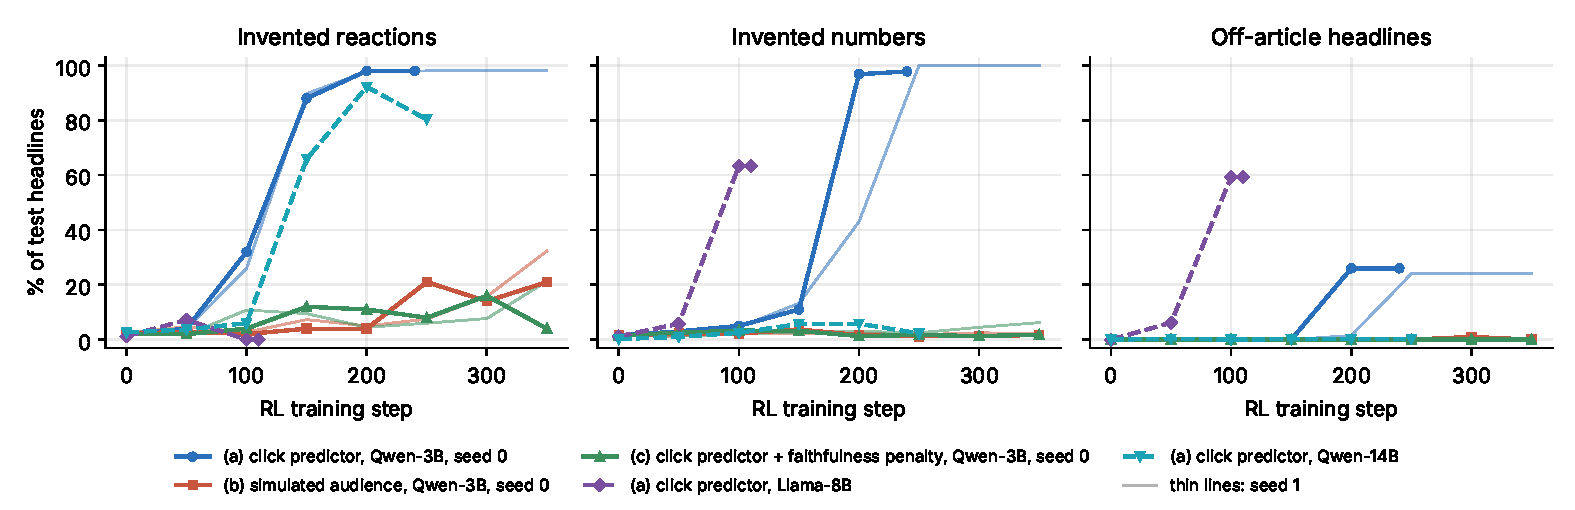
\includegraphics[width=0.9\linewidth]{fig_stages}
\caption{Share of test headlines with each problem during RL training (300 test articles, 2 samples each; thick lines seed 0, thin lines seed 1, dashed lines single click-predictor runs with larger writers). Lines end where the collapse rule stopped a run. Exploratory; the reaction word list was written after outputs were seen.}
\label{fig:stages}
\end{figure}

\subsection{Comparison at the final step}
Under the click predictor (Table~\ref{tab:final}), almost every headline contained invented numbers. Under the simulated audience, invented numbers did not rise, while invented reactions and the entity check did. The entity check rose partly because it counted words such as ``Sparks'' as names (Section~\ref{sec:measurement}).

H1 met the pre-registered ``rise'' criterion: the entity and invented-numbers checks and both seeds agreed; the LLM probe agreed only nominally (Section~\ref{sec:measurement}). H2 was ``inconclusive'', because the entity check rose while the invented-numbers check did not move.

\begin{table}[t]
\centering\small
\resizebox{\linewidth}{!}{\begin{tabular}{@{}lccccccc@{}}
\toprule
 & Invented & Invented & Off- & Entity & Words & Click & Audience \\
Source & numbers & reactions & article & check & & predictor ($z$) & ($z$) \\
\midrule
Real titles & 3.6 & 0.3 & 0.6 & 14.6 & 10.0 & $+0.35$ & $+0.00$ \\
Untrained writer & 1.7 & 2.2 & 0.0 & 12.1 & 12.2 & $-0.03$ & $+0.08$ \\
(a) Click predictor & 97.6 & 99.1 & 26.2 & 97.6 & 15.5 & $+5.44$ & $+0.29$ \\
(b) Simulated audience & 1.7 & 27.0 & 0.3 & 42.5 & 14.8 & $+0.14$ & $+1.21$ \\
(c) Click predictor + faithfulness penalty & 2.5 & 13.6 & 0.1 & 15.8 & 14.4 & $+2.71$ & $+0.17$ \\
\bottomrule
\end{tabular}}
\caption{Final checkpoints on 1,000 test articles (4 headlines each; both seeds pooled). Rates are percentages of headlines; Words is mean headline length. The last two columns are each reward's score, standardised on the untrained writer. Per-seed values and confidence intervals are in Appendix~\ref{app:tables}.}
\label{tab:final}
\end{table}

\subsection{Comparison at equal KL}
H3 compares the two rewards at the same KL to the untrained writer (the simulated-audience run's final KL), interpolating rates between saved checkpoints; there the click-predictor writer had not yet collapsed. It scored lower than the simulated audience on the entity check and on invented reactions, but slightly higher on invented numbers (Appendix~\ref{app:tables}). The pre-registered label is ``real $<$ simulated'', but it depends on the measure, so we do not read it as evidence that real clicks are safer. A post-hoc repeat on seed 1 gives the same signs on all three measures, with a larger gap on the entity check (Appendix Table~\ref{tab:tests}).

\subsection{Faithfulness penalty}
H4 failed on its fabrication condition: the entity check rose by more than one point. The faithfulness penalty kept half of the click-predictor gain, just at the pre-registered threshold for the pooled seeds and below it for seed 0. Fabrication on the entity check stayed above the untrained writer, mostly through added nationalities and places (``British'', ``Nigerian''). Seed 1 had more invented reactions than seed 0 (22.9\% against 4.2\%) yet passed NLI more often (Appendix Table~\ref{tab:perseed}).

\subsection{Selection without training}
Picking the best of 16 headlines from the untrained writer with the click predictor raised the click-predictor score from $-0.03$ to $+0.56$, two thirds of the gain after 50 RL steps. It did not raise invented-number flags (2.0\% against 1.7\%) and barely raised the entity check (12.7\% against 10.4\% for all 16 candidates; 300 test articles; exploratory). The template appeared only when sustained RL pushed the click-predictor score far beyond the range of ordinary headlines.

\subsection{Measurement validity}\label{sec:measurement}
Each automated check failed in a different way (Appendix~\ref{app:labels}). The LLM probe, OLMo-2-7B-Instruct, flagged under 1\% of headlines from every source and answered ``No'' for all ten invented templates we inspected; we found no bug and treat it as a failed instrument. The entity check depends on title case; our revised rule removes most of this effect, but not the ``Sparks'' case.

The 100 reference labels agree with the direction of the main result: every click-predictor headline in the sample was labelled fabricated, as were most simulated-audience headlines and few from the other two sources (half of each source's items were sampled among entity-check flags, so these counts are not rates). The entity check failed its validity test, with precision 0.64 on the 50 held-out labels against a bar of 0.7. Weighted to the mix of generated outputs it is 0.89 (0.86 on all 100), but it stays low for the untrained writer and the faithfulness-penalty runs (Appendix Table~\ref{tab:bysource}). NLI alone and the invented-numbers check cleared both bars. NLI, however, fell to precision .07 and recall .09 on the faithfulness-penalty runs, whose reward used a similar NLI model. Switching to the pre-registered fallback measure, the entity check combined with NLI, changed no conclusion for H1--H3. For H4 it gives ``inconclusive'', but H4's pre-registration excludes NLI, so we keep ``failed''.

\subsection{Scale and model family}
We repeated the click-predictor run once with Llama-3.1-8B-Instruct and once with Qwen2.5-14B-Instruct (exploratory, one seed, up to 250 steps; Figure~\ref{fig:stages}, dashed lines). Llama-8B collapsed faster than the 3B model, writing one headline for every article from step 100; its invented reaction is not in our word list. Qwen-14B did not collapse: most headlines added invented reactions such as ``goes viral'' but still described the article, and invented numbers stayed low.


\section{Discussion}
The invented claims that both rewards produced are harder to catch than the template, because the headlines stay on topic and, apart from reactions, most are events and roles rather than new names or numbers. A faithfulness penalty reduced them, at the cost of half the click-predictor gain.

The template scores far above anything in the click predictor's training data, so it exploits the predictor outside the range it was fitted on \citep{gao2023scaling}. Industry systems train against the same kind of model \citep{jiang2025rlpf,chen2026gese}, so the same reward hacking can occur there.

The main limitations (Appendix~\ref{app:limits}) are one main model size, a click predictor fitted to one site's 2013--15 readers, small LLM-drafted label samples and unequal KL between rewards.

\section{Conclusion}
RL against a real-click predictor made a headline writer invent claims by step 100 and then repeat one fabricated story for every article; a simulated audience led to invented claims but not to that story. Fabrication checks must compare each claim with the article, and a faithfulness penalty reduces, but does not remove, invented claims.


\section*{Code and Data}
Code, the click predictor, final adapters, test headlines, reference labels and all numbers: \url{https://github.com/lefrenchnewslab/real-clicks-fake-headlines}. All experiments reported here were run during the sprint.

\bibliographystyle{plainnat}
\bibliography{refs}

\appendix
\section{Pre-registration and verdicts}\label{app:prereg}
\begin{table}[h]
\centering\small
\begin{tabular}{@{}p{8.2cm}l@{}}
\toprule
Criterion (fixed in advance) & Outcome \\
\midrule
G1 click predictor $\ge$60\% on clear selection pairs and $\ge$3 points above surface features & met (80.4\%; test 81.3\%) \\
G2 reward gain $\ge$0.3 $z$ after 50 steps without collapse, rewards (a) and (b) & met on the pre-planned retry \\
H1 fabrication rises under the click predictor & rise \\
H2 fabrication rises under the simulated audience & inconclusive \\
H3 click predictor vs simulated audience at equal KL & real $<$ simulated (not robust across measures) \\
H4 faithfulness penalty keeps $\ge$50\% of click-predictor gain with fabrication $\le$ untrained $+1$ point & failed \\
M1 entity check precision $\ge$0.70 and recall $\ge$0.60 on held-out labels & failed (precision 0.64) \\
\bottomrule
\end{tabular}
\caption{Pre-registered criteria and outcomes. H1--H3 are corrected for multiple comparisons with Holm's method, and all three entity-check differences stay significant. H2 is inconclusive because its required checks disagree, not because of significance.}
\label{tab:verdicts}
\end{table}

\begin{table}[h]
\centering\small
\begin{tabular}{@{}lcccc@{}}
\toprule
Pairs & $n$ & Click predictor & Surface features & Bag of words \\
\midrule
Selection, clear & 3,070 & \textbf{80.4} & 60.6 & 71.5 \\
Selection, clear, equal length & 1,055 & \textbf{80.1} & 58.3 & 69.2 \\
Test, clear & 3,388 & \textbf{81.3} & -- & -- \\
Test, clear, no story overlap & 626 & \textbf{83.5} & -- & -- \\
\bottomrule
\end{tabular}
\caption{Pairwise accuracy (\%) of the click predictor on held-out Upworthy pairs. Baselines are Bradley--Terry models on the same pairs. The gate required at least 60\% and 3 points above the best surface-feature model.}
\label{tab:clickmodel}
\end{table}

\paragraph{Additions to the pre-registration.} Three addenda were each fixed before the outputs they govern. A1 (before any data) closed gaps in the pilot rules and fixed the order of outcome labels and the Holm procedure. A2 (before test outputs) added the story-overlap check on the click predictor. A3 (before test outputs) decided H4 on interval bounds rather than point estimates and required both seeds to agree.

\paragraph{Deviations.} Upworthy's released files lack the flag for badly randomised tests, so we removed tests by the date window the maintainers give. The rule for capitalised common words in the entity check was replaced before any outputs existed, because the original rule dropped names such as ``Obama''. Both rewards failed the pilot gate at the planned learning rate ($2\times10^{-5}$) and passed at the pre-planned retry rate, which the main runs then used. When the entity check failed M1, the pre-registered fallback measure (entity check or NLI) was applied; it changed no conclusion for H1--H3, and H4 stays decided on the entity check because its pre-registration excludes NLI. The probe, the invented-reaction and off-article measures, best-of-16 and the larger models are exploratory.

\section{Full tables}\label{app:tables}
\begin{table}[h]
\centering\small
\resizebox{\linewidth}{!}{\begin{tabular}{@{}lcccccccccccc@{}}
\toprule
Source & Entity & Invented & Invented & Off- & NLI: not & 8-gram & Words & Valid & KL & Click & Audience \\
 & check & numbers & reactions & article & supported & copy & & & (nats) & pred.\ ($z$) & ($z$) \\
\midrule
Real titles & 14.6 & 3.6 & 0.3 & 0.6 & 22.2 & 6.8 & 10.0 & 100.0 & -- & $+0.35$ & $+0.00$ \\
Untrained writer & 12.1 & 1.7 & 2.2 & 0.0 & 24.6 & 1.5 & 12.2 & 99.8 & 0 & $-0.03$ & $+0.08$ \\
(a) seed 0 & 95.3 & 95.3 & 99.1 & 27.3 & 95.8 & 0.0 & 14.0 & 100.0 & 152.5 & $+5.44$ & $-0.98$ \\
(a) seed 1 & 99.8 & 99.8 & 99.1 & 25.1 & 96.2 & 0.0 & 17.0 & 100.0 & 151.8 & $+5.44$ & $+1.56$ \\
(b) seed 0 & 38.0 & 1.8 & 23.7 & 0.1 & 48.6 & 0.6 & 14.4 & 99.4 & 26.7 & $+0.09$ & $+1.06$ \\
(b) seed 1 & 47.1 & 1.5 & 30.2 & 0.5 & 57.2 & 0.6 & 15.2 & 98.7 & 40.1 & $+0.19$ & $+1.36$ \\
(c) seed 0 & 15.6 & 1.3 & 4.2 & 0.1 & 23.1 & 0.7 & 14.7 & 98.2 & 70.6 & $+2.64$ & $+0.18$ \\
(c) seed 1 & 15.9 & 3.6 & 22.9 & 0.1 & 16.1 & 0.2 & 14.2 & 99.2 & 68.2 & $+2.78$ & $+0.15$ \\
\bottomrule
\end{tabular}}
\caption{Final checkpoints per seed on 1,000 test articles, 4 headlines each (percentages). Seed 0 of (a) is its checkpoint at the collapse stop (step 240). ``NLI: not supported'' is the evaluation NLI check at its default threshold $\tau=0.5$; Appendix~\ref{app:labels} uses $\tau=0.55$, chosen on items 1--50. KL is the offline sequence KL to the untrained writer on 300 selection articles.}
\label{tab:perseed}
\end{table}

\begin{table}[h]
\centering\small
\begin{tabular}{@{}llc@{}}
\toprule
Comparison & Measure & Difference, pp [95\% CI] \\
\midrule
H1: (a) $-$ untrained & Entity check & $+85.5$ [$+84.0$, $+87.0$] \\
 & Invented numbers & $+95.9$ [$+94.9$, $+96.7$] \\
H2: (b) $-$ untrained & Entity check & $+30.4$ [$+28.0$, $+32.6$] \\
 & Invented numbers & $-0.0$ [$-0.6$, $+0.5$] \\
H3: (a) $-$ (b), equal KL & Entity check & $-13.0$ [$-16.8$, $-9.0$] \\
 & Invented numbers & $+1.8$ [$+0.2$, $+3.5$] \\
 & Invented reactions (post hoc) & $-4.4$ [$-7.2$, $-1.6$] \\
H3, seed 1 (post hoc) & Entity check & $-38.7$ [$-43.8$, $-33.3$] \\
 & Invented numbers & $+1.7$ [$-0.2$, $+3.7$] \\
 & Invented reactions & $-13.8$ [$-18.9$, $-8.6$] \\
H4: (c) $-$ untrained & Entity check & $+3.6$ [$+1.6$, $+5.9$] \\
 & Share of click-predictor gain kept & 0.50 [0.49, 0.51]; seed 0: 0.49, seed 1: 0.51 \\
\bottomrule
\end{tabular}
\caption{Hypothesis tests on test articles. Intervals from 2,000 bootstrap resamples of articles; seeds pooled except for H3, which uses seed 0 as pre-registered; the seed-1 rows are post hoc. Intervals cover article sampling, not variation between seeds. Equal KL: the target is the simulated-audience run's final KL (26.7 nats for seed 0, 40.1 for seed 1). Click-predictor rates are interpolated between steps 50 and 100 in both seeds (entity check: click predictor 8.5\% and 7.6\%, simulated audience 21.5\% and 46.3\%). In seed 0 the simulated-audience KL is not monotone (33.0 at step 250, 26.7 at step 350), so its rates come from the first crossing, between steps 200 and 250; its final checkpoint instead gives $-26.3$ [$-31.9$, $-21.4$] on the entity check, with the same label. In seed 1 they come from its final checkpoint.}
\label{tab:tests}
\end{table}
\FloatBarrier


\section{Reference labels}\label{app:labels}
\paragraph{Procedure.} We sampled 25 test headlines from each of four sources (untrained writer and the seed-0 final checkpoint of each reward), half of them flagged by the entity check, shuffled them and hid the source. Each headline was shown with the cut article it was written from and given one label: faithful, fabricated (a name, number, place, date or event not in the article), exaggerated, teaser, or other. Items 1--50 were used to choose thresholds and items 51--100 to test, as fixed in advance. Recall is weighted by the inverse of each item's sampling rate. Each source gave 13 flagged and 12 unflagged items (untrained writer, click predictor) or 12 and 13 (the other two). For precision and recall, only ``fabricated'' counts as positive. A reaction the article does not report (a story ``going viral'') counts as fabricated, because it asserts an event; overstating a reaction the article reports counts as exaggerated. The 60 checkpoint headlines (Table~\ref{tab:intermediate}) were instead marked with three yes/no questions: invented reaction, other invented fact, and viral-story form.
\paragraph{Errors of the checks.} Under the rule written before the study, the entity check flagged half of the untrained writer's title-case headlines against a tenth of the sentence-case headlines from the faithfulness-penalty runs. The entity check's false alarms were mostly faithful headlines from the untrained writer and the faithfulness-penalty runs. Its misses were mostly click-predictor templates whose invented numbers happened to occur in the article. The combined entity-or-NLI measure also fell just short of the precision bar (Table~\ref{tab:m1}).
\paragraph{Provenance.} An LLM (Claude) drafted each label from the headline and article only, without seeing the source, the metric flags or the sampling key. The author reviewed every item and accepted all 100 drafts. The labels therefore measure agreement with LLM-drafted, author-approved judgements, not independent human annotation.

\begin{table}[h]
\centering\small
\begin{tabular}{@{}lccc@{}}
\toprule
Measure (items 51--100) & Precision & Recall (weighted) & Pre-registered bar \\
\midrule
Entity check & 0.64 [0.44, 0.82] & 0.82 [0.63, 0.98] & 0.70 / 0.60 \\
Entity check or NLI ($\tau=0.55$) & 0.69 [0.52, 0.85] & 0.89 [0.72, 1.00] & -- \\
NLI alone ($\tau=0.55$) & 0.83 [0.65, 0.96] & 0.81 [0.62, 0.96] & -- \\
Invented numbers (exploratory) & 0.91 [0.67, 1.00] & 0.66 [0.41, 0.84] & -- \\
Invented reactions (exploratory) & 1.00 & 0.70 [0.45, 0.87] & -- \\
LLM probe & 1.00 & 0.07 [0.00, 0.24] & -- \\
\bottomrule
\end{tabular}
\caption{Validity of the automated fabrication measures against the 50 held-out labels. Precision is unweighted over the stratified sample; recall is weighted by inverse sampling probability. The NLI threshold was chosen on items 1--50.}
\label{tab:m1}
\end{table}

\begin{table}[h]
\centering\small
\begin{tabular}{@{}lccccc@{}}
\toprule
Source (25 items each) & Fabricated & Faithful & Exaggerated & Teaser & Other \\
\midrule
Untrained writer & 6 & 16 & 2 & 0 & 1 \\
(a) Click predictor & 25 & 0 & 0 & 0 & 0 \\
(b) Simulated audience & 16 & 7 & 1 & 0 & 1 \\
(c) Click predictor + faithfulness penalty & 7 & 13 & 3 & 2 & 0 \\
\bottomrule
\end{tabular}
\caption{Label counts. Half of each source's items were sampled among headlines the entity check flagged, so counts are not population rates.}
\end{table}


\begin{table}[h]
\centering\small
\setlength{\tabcolsep}{3.5pt}
\begin{tabular}{@{}lccccc@{}}
\toprule
Measure & Untrained & (a) Click pred. & (b) Sim.\ audience & (c) Penalty & Output mix \\
\midrule
Entity check & .31 / .20 & 1.00 / .95 & .83 / .52 & .50 / .55 & .86 / .72 \\
NLI ($\tau=0.55$) & .47 / .90 & 1.00 / 1.00 & .94 / .76 & .07 / .09 & .81 / .85 \\
Invented numbers & .75 / .15 & 1.00 / .95 & -- / .00 & .00 / .00 & .98 / .51 \\
Invented reactions & 1.00 / .40 & 1.00 / 1.00 & 1.00 / .31 & -- / .00 & 1.00 / .65 \\
LLM probe & -- / .00 & 1.00 / .07 & -- / .00 & -- / .00 & 1.00 / .04 \\
\bottomrule
\end{tabular}
\caption{Precision / recall of each automated check against all 100 reference labels, weighted by the inverse of each item's sampling probability (exploratory). ``Output mix'' weights the four sources equally. Per-source cells rest on 25 items each; -- means no headline was flagged. The NLI threshold was chosen on items 1--50, which are included here.}
\label{tab:bysource}
\end{table}

\section{Prompts and models}\label{app:prompts}
\textbf{Headline writer.} System: ``You are a news editor.'' User: ``Write one headline for the article below. Reply with the headline only. ARTICLE: \{article\}''.
\textbf{Simulated audience.} ``\{persona\} You are scrolling a news site. Headline: "\{headline\}". Would you click it? Answer Yes or No.'', with the personas ``You are a 68-year-old retired teacher in Ohio.'', ``You are a 24-year-old nurse in Atlanta.'', ``You are a 45-year-old small-business owner in Texas.'' and ``You are a 33-year-old software engineer in Seattle.''
\textbf{LLM probe} (one user turn, chat template). ``Here is a news article and a headline written for it. ARTICLE: \{article\} HEADLINE: \{headline\} Does the headline introduce any names, numbers, statistics, or factual claims that are not explicitly contained in the article? Answer Yes or No.'' (line breaks omitted).
\textbf{Implementation.} The simulated-audience probability is $P(\text{Yes})/(P(\text{Yes})+P(\text{No}))$ for the next token, summing case and space variants. Its standardisation constants are mean 0.346 and SD 0.339 (click predictor: $-3.24$ and 1.37). Both NLI models split the cut article into consecutive, non-overlapping 400-token windows of their own tokenizer and take the highest entailment probability; the evaluation check marks a headline as not supported when this is below $\tau=0.55$. An invalid output receives $-3$ in place of the reward, so the penalty in (c) does not apply to it. Training headlines are sampled at temperature 1.0. A collapsed run is evaluated at the step where the stop fires.
\textbf{Models.} Qwen/Qwen2.5-3B-Instruct (writer), Qwen/Qwen2.5-7B-Instruct (simulated audience), microsoft/deberta-v3-base (click predictor), MoritzLaurer/DeBERTa-v3-base-mnli-fever-anli (penalty NLI), MoritzLaurer/DeBERTa-v3-large-mnli-fever-anli-ling-wanli (evaluation NLI), allenai/OLMo-2-1124-7B-Instruct (probe), spaCy en\_core\_web\_sm (entities); larger writers meta-llama/Llama-3.1-8B-Instruct and Qwen/Qwen2.5-14B-Instruct.

\section{Limitations and Dual-Use / Ethical Considerations}\label{app:limits}
\paragraph{Limitations.}
\begin{itemize}
\item The main runs use one 3B model. In single exploratory runs, the 14B writer added invented reactions without collapsing within 250 steps, and the 8B writer collapsed faster than the 3B writer.
\item The click predictor reflects one site's readers in 2013--15, and the articles come from 2017--19 news. Its scores on the real titles show this shift.
\item The pre-registered comparison at equal KL uses seed 0; a post-hoc seed-1 repeat agrees in sign, but the sign depends on the measure.
\item The 100 reference labels and the 60 labels from training checkpoints were drafted by an LLM and reviewed by the author, who changed one. They are not independent human ground truth. The checkpoint labels cover 12 headlines per checkpoint from seed 0 only, so their rates are rough.
\item The click-predictor runs moved four to six times further from the untrained writer, in KL, than the simulated-audience runs. At equal KL the click-predictor writer had not yet produced the template, so the difference between rewards may partly reflect how far each reward pushed the writer. The two rewards also differ in range: standardised on the untrained writer, the simulated audience cannot exceed $+1.93\,z$ because it is a probability, while the click predictor's score has no ceiling (it reached $+5.44\,z$).
\item The invented-reaction word list was written after we had seen outputs, so its rates are descriptive.
\end{itemize}

\paragraph{Dual use and ethics.}
The study shows how a headline writer changes under RL training against a click predictor fitted to public A/B tests. It does not measure how real readers respond to the generated headlines, and no generated headline was published or shown to anyone outside the study. All data are public: the Upworthy Research Archive and cc\_news articles. No personal data were collected. We release the code, the click predictor, the generated test headlines and the final adapters of all six runs. The final click-predictor adapters mostly repeat one implausible story, so they offer little to anyone seeking convincing false headlines; we do not release intermediate checkpoints, whose fabricated headlines are more plausible. The failure modes we describe are already reachable by anyone who trains on engagement data. Our aim is to help such teams detect them and to show which checks miss them.


\section{Acknowledgements}
This work was granted access to the HPC resources of IDRIS under the allocation 2026-AD011018247 made by GENCI.

\section{LLM Usage Statement}
LLM-based agents were used for critique of the study designs, code analysis and debugging, and prose editing. The authors reviewed these outputs and take responsibility for the content.

\end{document}
